\title{Rękawiczka sensoryczna}
\documentclass[12pt, a4paper]{article}

\usepackage{amsmath}
\usepackage{amsfonts}
\usepackage{graphicx}
\usepackage{float}
\usepackage{listings}
\usepackage{multicol}
\usepackage{subcaption}
\usepackage{csquotes}
\usepackage{hyperref}
\usepackage{rotating}

\setlength\parindent{0pt}

\title{Systemy zdarzeniowe}
\usepackage[T1]{fontenc}
\usepackage[polish]{babel}
\usepackage[utf8]{inputenc}
\usepackage{lmodern}
\usepackage{geometry}
\usepackage{titling} %do ustawiania strony tytulowej na srodku
\renewcommand\maketitlehooka{\null\mbox{}\vfill} %i to
\renewcommand\maketitlehookd{\vfill\null}% i to
\usepackage{graphicx} %do dodawania zdjec w formatach PNG, JPG, EPS, PDF
\def\changemargin#1#2{\list{}{\rightmargin#2\leftmargin#1}\item[]} %umozliwi tymczasowa zmiane marginesow 
\let\endchangemargin=\endlist %przydatne przy wstawianiu tabel i zdjec
\usepackage{pdfpages}
\selectlanguage{polish}

\author{Jakub TACZAŁA\\Piotr GOGOLA\\Krzysztof DANIELAK\\Wojciech KOSICKI}

\vfill
\date{\today}
\begin{document}
\def\tablename{Tabela}
\begin{titlingpage}
\maketitle
\end{titlingpage}
\newpage
\tableofcontents %automatyczny spis treści
\newpage
\section{Problem projektu}
\label{sec:problem_projektu} %definicja etykiety rozdzialu

\subsection{Nazwa projektu} % deklaracja podrozdziału
\label{subsec:nazwa_projektu}         % deklaracja etykiety podrozdziału
Ratowniczy system przeszukiwania pomieszczeń.
\subsection{Opis ogólny} 
\label{subsec:opis_ogolny} 
Głównym celem projektu jest opracowanie zdarzeniowego systemu ratowniczego opartego o jednostkę centralną oraz rój autonomicznych robotów poszukiwawczych. Kształt pomieszczeń będzie znany poprzez wprowadzenie do centrali planu budynku. Do celów projektowych zostanie stworzony podprogram do tworzenia planu budynku i przetwarzania go do postaci potrzebnej do obsługi programu. Roboty w roju będą posiadać niezależne oprogramowanie służące do poruszania się po wyznaczonym terenie oraz do informowania o znalezionych ludziach. Roboty będą podawać swoje położenie do centrali w celu uzyskania pozwolenie na dotarcie do danego punktu. Planowane jest uzyskanie ruchu ciągłego przez roboty.

\subsection{Zastosowanie} 
\label{subsec:zastosowanie}        
System będzie wykorzystywany do przeszukiwania pomieszczeń, np. w czasie pożaru, by nie narażać ratowników na utratę zdrowia bądź życia.

\subsection{Założenia projektowe} 
\label{subsec:zalozenia_projektowe}
\begin{itemize}
    \item Stały plan;
    \item Ruch ciągły roju;
    \item Roboty nie znają ilości poszukiwanych osób, muszą przeszukać cały teren;
    \item Rozmieszczenie pomieszczeń i poszukiwanych osób zostaje zadawane przed symulacją poprzez wgranie odpowiedniego planu budynku;
    \item Pomimo wstępnie planowanej ścieżki roboty muszą unikać kolizji (możliwość zderzenia, zablokowania);
    \item Każdy robot posiada własną jednostkę sterującą;
    \item Opracować sposób wymijania się.
\end{itemize}

\subsection{Spodziewane wyniki pracy} 
\label{subsec:spodziewane_wyniki_pracy}         
Zakładane jest uzyskanie symulacji systemu pozwalającego na przeszukiwanie pomieszczeń. System poprzez symulacje pozwoli także oszacować skuteczna ilość robotów w roju podczas konkretnego zadania.

\subsection{Cel projektu} 
\label{subsec:cel_projektu}         
Celem projektu jest uzyskanie oprogramowania symulującego system zdarzeniowy złożony z roju autonomicznych robotów i sterownika centralnego, których zadaniem jest przeszukiwanie budynków w celu odszukania poszkodowanych w sytuacjach zagrażających życiu.

\subsection{Środowisko i narzędzia programistyczne} 
\label{subsec:srodowisko_i_narzędzia_programistyczne} 
Oprogramowanie zostanie wytworzone z wykorzystaniem następujących narzędzi:
\begin{itemize}
    \item Język programowania: Python 3.6.8;
    \item Menadżer pakietów dla Python 3.6: pip;
    \item Testy jednostkowe: pytest;
    \item Budowa interfejsu graficznego: PyQt5;
    \item System zarządzania kontrolą wersji: GIT;
    \item Środowisko: PyCharm lub Visual Studio Code;
    \item Tworzenie raportów: System składni tekstu \LaTeX{}, platforma Overleaf.com.
\end{itemize}

\subsection{Sposób upowszechnia} 
\label{subsec:Sposob_upowszechnia}  
Etapy realizacji projektu oraz efekt końcowy wraz z użytym oprogramowaniem 
i dokumentacjami będą dostępne poprzez dostęp do repozytorium publicznego serwisu GitHub pod adresem:\\ https://github.com/PiotrGog/SystemyZdarzeniowe.
\subsection{Sposób prezentacji wyników projektu} 
\label{subsec:sposob_prezentacji_wyników_projektu}        
Projekt będzie zaprezentowany poprzez prezentacje symulacji komputerowej dla różnych przypadków.\newpage
\section{Plan pracy i rozkład w czasie}
\label{sec:plac_pracy_kamienie_milowe_i_rozklad_w_czasie} %definicja etykiety rozdzialu
\subsection{Plan pracy}
\begin{table}[h!]
\begin{center}
\begin{tabular}{|p{6cm}|p{2.2cm}|p{2.2cm}|p{3.2cm}|} % deklaracja tabeli złożonej z 4 kolumn
\hline
Nazwa zadania & Data rozpoczęcia & Data zakończenia & Wykowawca \\ \hline
Rozpoznanie projektowe & 2019-10-03 & 2019-10-10 & Cała grupa\\ \hline
Opracowanie założeń & 2019-10-10 & 2019-10-17 & Krzysztof Danielak, Jakub Taczała, Wojciech Kosicki\\ \hline
Analiza dostępnych środowisk & 2019-10-10 & 2019-10-17 & Piotrek Gogola \\ \hline
Opracowanie algorytmu ogólnego & 2019-10-17 & 2019-10-24 & Jakub Taczała\\ \hline
Opracowanie systemu generowania mapy & 2019-10-17 & 2019-10-24 & Piotrek Gogola, Wojciech Kosicki\\ \hline
Opracowanie algorytmu szczegółowego centrali  & 2019-10-24 & 2019-11-14 & Wojciech Kosicki\\ \hline
Opracowanie algorytmu szczegółowego robota roju  & 2019-10-24 & 2019-11-14 & Krzysztof Danielak\\ \hline
Implementacja jednostki centralnej & 2019-11-14 & 2019-11-28 & Piotrek Gogola,  Wojciech Kosicki\\ \hline
Implementacja osobnika roju & 2019-11-14 & 2019-11-28 & Krzysztof Danielak, Jakub Taczała\\ \hline
Scalenie roju z jednostką centralną & 2019-11-28 & 2019-12-05 &  Cała grupa\\ \hline
Testy na pojedynczym osobniku & 2019-12-05 & 2019-12-12 &  Cała grupa\\ \hline
Testy na wielu osobnikach & 2019-12-12 & 2019-12-20 &  Cała grupa\\ \hline
Wprowadzenie poprawek & 2019-12-20 & 2020-01-09 &  Cała grupa\\ \hline
Stworzenie ostatecznej dokumentacji projektowej & 2020-01-09 & 2020-01-16 &  Cała grupa\\ \hline
\end{tabular}.
\end{center}
\caption{\label{rj}Zadania} % Nadanie etykiety
% tablicy (\label{rj}) i jej opis.
\end{table}\newpage
\section{Doręczenia i kamienie milowe}
\label{sec:doreczenie} %definicja etykiety rozdzialu
\begin{table}[h]
\begin{center}
\begin{tabular}{|p{8cm}|l|p{2.5cm}|}
\hline 
Kamień milowy & Data & Doręczenia \\ \hline
Opracowanie algorytmów ogólnych & 24 październik 2019 & raport \\ \hline
Opracowanie algorytmów szczegółowych & 14 listopad 2019 & raport \\ \hline
Implementacja kodu jednostki centralnej i pojedynczego osobnika roju & 28 listopad 2019 & raport \\ \hline
Przeszukiwanie terenu przez jednego robota & 05 grudzień 2019 & raport \\ \hline
Bezkolizyjne przeszukiwanie terenu przez rój robotów & 20 grudzień 2019 & raport \\ \hline
Wizualizacja zachowania robotów w symulacji & 09 styczeń 2020 & raport \\ \hline
Demonstracja działania symulacji & 16 styczeń 2020 & raport, prezentacja projektu \\ \hline
\end{tabular}
\end{center}
\caption{\label{rj}Terminy doręczeń} % Nadanie etykiety
\end{table} \newpage
%\section{Budżet}
\label{sec:budzet} %definicja etykiety rozdzialu
\begin{table}[hbt]
\begin{center}
\begin{tabular}{|l|p{5cm}|p{1.4cm}|p{1.4cm}|l|p{1.6cm}|p{1.6cm}|}
\hline 
Lp. & Nazwa & Cena netto & Cena brutto & Ilość & Cena netto w sumie & Cena brutto w sumie \\ \hline
1	&STM32F100C8T6B - LQFP48	 &8,93  zł 	 &10,99  zł 	&2,00	 &17,87  zł 	 &21,98  zł \\ \hline
2	&Moduł nRF24L01+ 2.4GHz wireless	 &4,71  zł 	 &5,79  zł 	&3,00	 &14,12  zł 	 &17,37  zł \\ \hline
3	&Czujnik siły nacisku okrągły 5mm (0,25'') - krótkie złącze	 &23,10  zł 	 &28,41  zł 	&5,00	 &115,49  zł 	 &142,05  zł \\ \hline
4	&Czujnik ugięcia 73x6,3mm - SparkFun	 &31,63  zł 	 &38,90  zł 	&5,00	 &158,13  zł 	 &194,50  zł \\ \hline
5	&Ładowarka Li-Pol TP4056 pojedyncza cela 1S 3,7V microUSB z zabezpieczeniami	 &6,42  zł 	 &7,90  zł 	&2,00	 &12,85  zł 	 &15,80  zł \\ \hline
6	&Pakiet Li-Pol 3.7V 550mAh	 &14,30  zł 	 &17,59  zł 	&2,00	 &28,60  zł 	 &35,18  zł \\ \hline
7	&Laminat światłoczuły 100x150x1.5mm jednostronny +	 &11,37  zł 	 &13,99  zł 	&1,00	 &11,37  zł 	 &13,99  zł \\ \hline
8	&Rękawiczki długie BRUBECK Smart Gloves	 &32,44  zł 	 &39,90  zł 	&1,00	 &32,44  zł 	 &39,90  zł \\ \hline
9	&Wysyłka electropark.pl	 &8,93  zł 	 &10,99  zł 	&1,00	 &8,93  zł 	 &10,99  zł \\ \hline
10	&Wysyłka botland.com.pl	 &12,11  zł 	 &14,90  zł 	&1,00	 &12,11  zł 	 &14,90  zł \\ \hline
11	&Wysyłka centrumrowerowe.pl	 &11,37  zł 	 &13,99  zł 	&1,00	 &11,37  zł 	 &13,99  zł   \\ \hline 
$\Sigma$ & Podsumowanie & & & & & 520,65zł\\ \hline        
\end{tabular}
\end{center}
\caption{\label{rj}Koszty} % Nadanie etykiety
\end{table}
\begin{flushleft}
\end{flushleft}


 \newpage
\section{Zarządzanie projektem}
\label{sec:zarzadzanie_projektem} %definicja etykiety rozdziału
Wszelkie konflikty zaistniałe podczas realizacji projektu będą rozwiązywane poprzez ostateczną decyzję koordynatora projektu po wcześniejszej rozmowie z członkami zespołu. Projekt będzie powstawał pod ciągłą kontrolą postępów pracy, co pozwoli na równoległe rozwiązywanie zaistniałych problemów.

Koordynator zespołu ma możliwość ocenienia pracy każdego z członków poprzez uwzględnienie jego zaangażowania. Zadaniem koordynatora jest przydzielenie poszczególnych zadań, weryfikacja jakości, postępu oraz możliwość modyfikacji w razie takiej konieczności. Rolą koordynatora jest także motywacja, wsparcie mentalne i merytoryczne oraz rozwijanie umiejętności miękkich wśród reszty grupy projektowej.

Postępy prac będą monitorowane poprzez odgórny nadzór koordynatora poprzez raporty ustne, oraz wgląd w postęp prac. Z zebranych informacji koordynator będzie tworzył raporty postępu prac, które będą publikowane za pośrednictwem programu E-portal.pl. Raporty składowane będą na platformie overleaf.com, która pozwala na edycję dokumentów pisanych w składni {\LaTeX} przez wielu użytkowników jednocześnie. Kod źródłowy oprogramowania będzie składowany przez serwis github.com.

Każde zadanie przed realizacja zostanie omówione, oraz zostaną określone cele jego realizacji. Następnie po stworzeniu danego modułu i poddaniu go testom zostanie omówiony wynik, na podstawie którego zostanie stworzony raport.  \newpage
\section{Zespół}
\label{sec:zespol} %definicja etykiety rozdzialu
\label{subsec:pozostali_czlonkowie_grupy}
\begin{table}[hbt]
\begin{center}
\begin{tabular}{|c|c|c|p{6.2cm}|} % deklaracja tabeli złożonej z 4 kolumn
\hline
Nazwisko & Imię & Numer indeksu & Przydzielone zadania \\ \hline
TACZAŁA & Jakub & 226495 & Koordynator projektu,  opracowanie ogólnego algorytmu działa systemu. Prowadzenie sprawozdań, pomoc przy implementacji.\\ \hline
GOGOLA & Piotr & 226249 &  Główny programista, przygotowanie środowiska programistycznego, scalenie modułów programu.\\ \hline
KOSICKI & Wojciech & 234506 & Opracowanie szczegółowego algorytmu działania jednostki centralnej. Pomoc przy implementacji.\\ \hline
DANIELAK &Krzysztof& 229081 &  Opracowanie szczegółowego algorytmu pracy pojedynczego robota.  Pomoc przy implementacji.\\
\hline
\end{tabular}
\end{center}
\caption{\label{rj}Podział zadań} % Nadanie etykiety
\end{table} 
\section{Definiowanie planu w postaci mapy}
Dozwolona przestrzeń zewnętrzna poruszania się robotów zdefiniowana jest poprzez mapę reprezentowaną w postaci dwuwymiarowej tablicy, gdzie odpowiednie wartości określają ściany, poszukiwane obiekty (ranni ludzie), stany dozwolone, stany zakazane i inne. Mapy generowane są za pomocą programu \href{https://www.mapeditor.org/}{Tiled}. Interfejs programu został przedstawiony na Rys. \ref{fig:tiled}.
\begin{figure}[H]
    \centering
    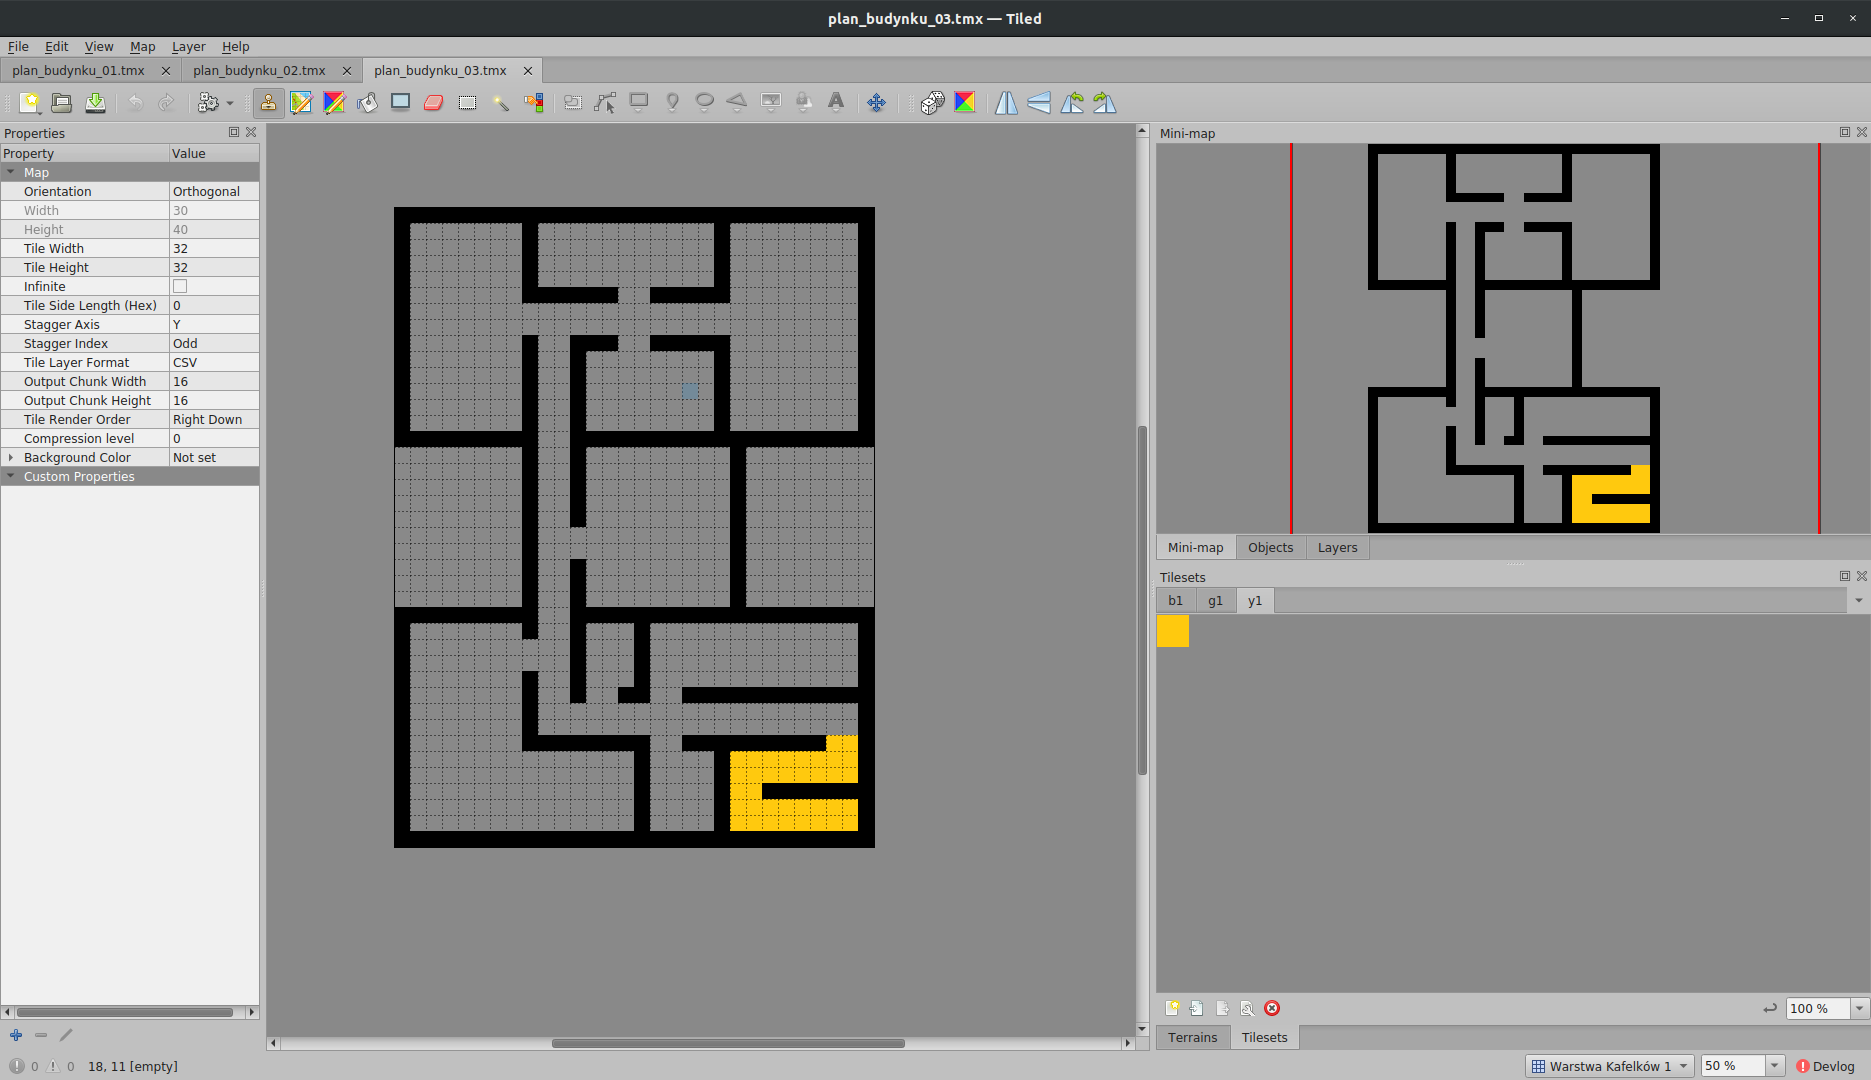
\includegraphics[width=0.7\textwidth]{figures/tiled}
    \caption{Okno edytora map 2D \textit{Tiled}}
    \label{fig:tiled}
\end{figure}

Rys. \ref{fig:mapy} przedstawia przykładowe, utworzone w celach testowych mapy.
\begin{figure}[H]
    \centering
    \begin{subfigure}[b]{0.3\textwidth}
        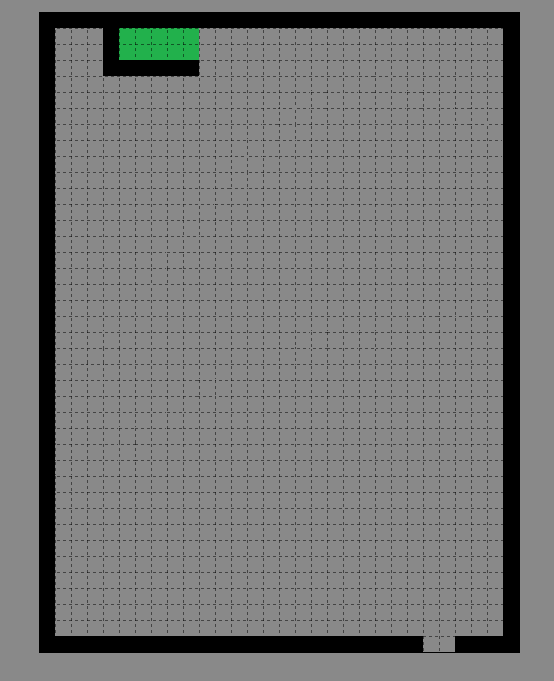
\includegraphics[width=\textwidth]{figures/p1.png}
        \caption{}
        \label{fig:gull}
    \end{subfigure}
    ~
    \begin{subfigure}[b]{0.3\textwidth}
        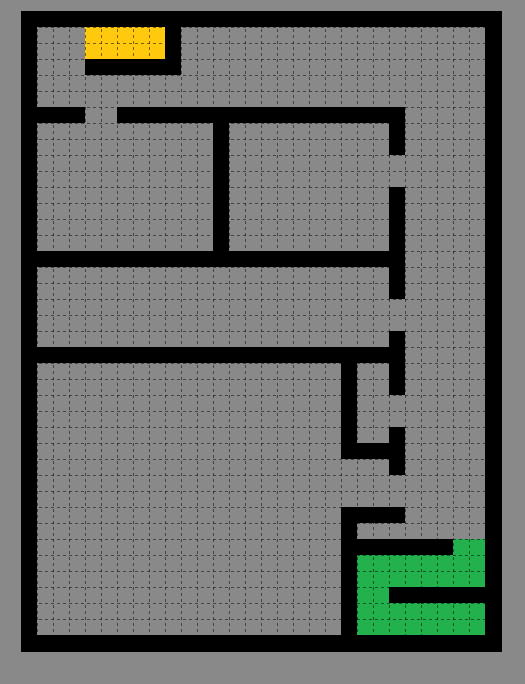
\includegraphics[width=\textwidth]{figures/p2.png}
        \caption{}
        \label{fig:tiger}
    \end{subfigure}
    ~
    \begin{subfigure}[b]{0.3\textwidth}
        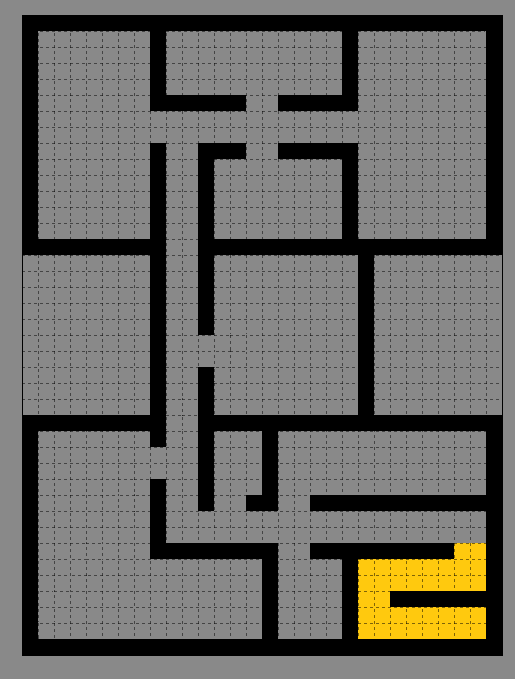
\includegraphics[width=\textwidth]{figures/p3.png}
        \caption{}
        \label{fig:mouse}
    \end{subfigure}
    \caption{Przykładowe mapy o różnym stopniu złożoności}
    \label{fig:mapy}
\end{figure}

Zielone i pomarańczowe obszary oznaczają odpowiednio schody w górę i w dół.\\
\\
Osoby poszkodowane rozmieszczane są poprzez funkcję \textit{random} w losowych miejscach. Ilość poszkodowany ustalana jest każdorazowo odgórnie do celów symulacji. Położenie oraz ilość celi nie są znane dla jednostki centralnej oraz roju robotów poszukiwawczych.\\
\\
Po przygotowaniu map są one eksportowane do pliku w formacie *.json. Plik ten zawiera wyeksportowaną mapę zapisywaną w postaci jednowymiarowej tablicy i inne dane dotyczące planu. Plik następnie jest parsowany za pomocą skryptu w celu uzyskania dwuwymiarowej reprezentacji mapy i możliwości zapisu jej w postaci tekstowej (np.\@ w celu wyświetlenia, ręcznej edycji mapy) lub w postaci binarnej. Sparsowana mapa jest plikiem wejściowym do programu. Jednostka centralna pobiera dane o ściana, dzięki czemu ma możliwość wyznaczenia celów przeszukiwania oraz wstępnych tras dla robotów.
\section{Projekt systemu zdarzeniowego}
\subsubsection{Założenia sterownika nadrzędnego}
\label{subsec:sterownik_podrzedny_stany}
\begin{itemize}
    \item Sterownik centralny ma wprowadzoną przez operatora mapę terenu.
    \item Sterownik centralny wydaje pozwolenie wjazdu na dane pole.
    \item Sterownik centralny określa ścieżkę dla każdego robota.
    \item Sterownik centralny gromadzi informacje o odnalezionych celach (poszkodowanych).
    \item Sterownik zwraca informacje o przeszukaniu całej mapy.
\end{itemize}

\subsubsection{Założenia robota podrzędnego}
\begin{itemize}
    \item Pojedynczy robot podczas postoju zajmuje obszar 1x1.
    \item Robot obserwuje otoczenie na obszarze 3x3.
    \item Robot podczas poruszania się na wprost chwilowo zajmuje dwie działki (2x1).
    \item Możliwość obrotu o krotności kąta prostego.
    \item Priorytetem robotów jest unikanie kolizji.
    \item W przypadku konfliktu przejazdu centrala szuka najbliższego miejsca do wyminięcia.
    \item Wykrycie poszkodowanego nie zmienia zaplanowanej trasy
    \item Wykryta przeszkoda jest traktowana jako ściana
\end{itemize}

\subsection{Stan systemu}
Stan systemu reprezentowany jest poprzez listę par $(n, s)$, oznaczających: n -- indeks kroku danego robota, s -- stan przemieszczania się robota.
Przykładowa reprezentacja stanu wszystkich robotów: \\
$$S = [(9, j), (3, s), (10, s), (28, j)]$$
Oznacza, że pierwszy robot zmierza do osiągnięcia 9.\@ pozycji w zaplanowanej ścieżce, drugi robot stoi na 3.\@ pozycji, trzeci robot stoi na 10.\@ pozycji, a czwarty robot zmierza do 28.\@ pozycji.

\subsection{Zdarzenia}
$e_{i1}$ -- robot i-ty dojechał do kolejnej pozycji,\\
$e_{i2}$ -- robot i-ty wykrył przeszkodę,\\
$e_{i3}$ -- robot i-ty wykrył poszkodowanego,\\
$e_{i4}$ -- robot i-ty otrzymuje polecenie: jedź.\\

\subsection{Funkcje tranzycji}
f(($l_{ij}$, j), $e_{i1}$) = ($l_{ij}$, s)\\
f(($l_{ij}$, s), $e_{i2}$) = ($l_{ij}$, s)\\
f(($l_{ij}$, s), $e_{i3}$) = ($l_{ij}$, s)\\
f(($l_{ij}$, s), $e_{i4}$) = ($l_{ij+1}$, j)\\

\subsection{Możliwe następstwa stanów}
$\Gamma(l_{ij}, j)=\{e_{i1}\}$\\
$\Gamma(l_{ij}, s)=\{e_{i2}, e_{i3}, e_{i4}\}$

\subsection{Reprezentacja zaplanowanej ścieżki}
Dla każdego robota zaplanowana ścieżka będzie reprezentowana jako lista kolejnych współrzędnych definiujących następną lokalizację robota. Zestaw tak opisanych ścieżek dla wszystkich robotów będzie reprezentowany w postaci tablicy złożonej z $n$ list (n -- liczba robotów).

Przykładowa reprezentacja:
\begin{verbatim}
V = [
    [wsp_11, wsp_12, wsp_13, ... ], // dla 1. robota
    [wsp_21, wsp_22, wsp_23, ... ], // dla 2. robota
    [wsp_31, wsp_32, wsp_33, ... ], // dla 3. robota
    ...
    [wsp_i1, wsp_i2, wsp_i3, ... ], // dla i-tego robota
    ...
    [wsp_n1, wsp_n2, wsp_n3, ... ], // dla n-tego robota
]
\end{verbatim}
gdzie $wsp_{ij}$ prezentuje współrzędne w przestrzeni w postaci (piętro, współrzędna X, współrzędna Y).
\subsection{Graf algorytmu sterownika nadrzędnego}

\begin{figure}[H]
    \centering
    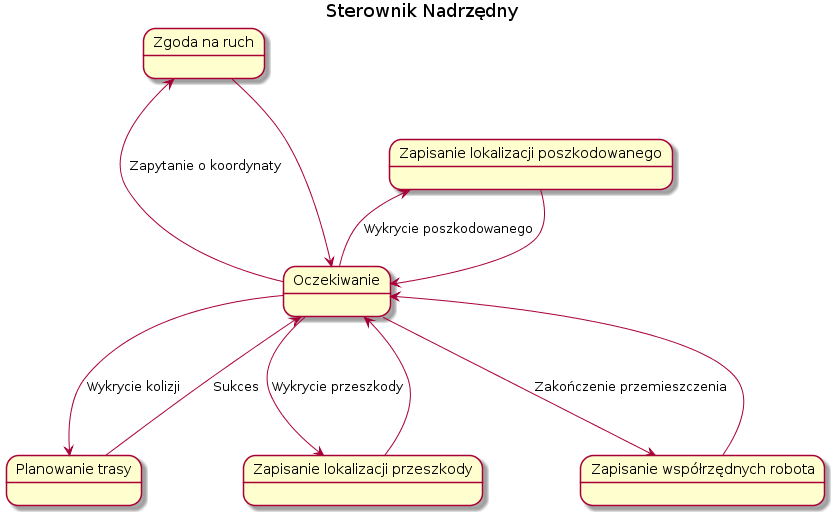
\includegraphics[width=1\textwidth]{gggg.png}
    \caption{Graf algorytmu sterownika nadrzędnego.}
    \label{fig:tiled}
\end{figure}

\newpage
\section{Szczegółowy opis działania elementów systemu}
\subsection{Działanie sterownika nadrzędnego}

\subsubsection*{Planowanie trasy}
\begin{enumerate}
    \item Pobierz aktualny stan mapy oraz poprzednio utworzoną listę kroków trasy każdego z robotów,
    \item Zaplanuj nowe ścieżki robotów,
    \item Uaktualnij listę kroków ścieżek robotów,
    \item Roześlij nowe ścieżki odpowiednio każdemu robotowi.
\end{enumerate}

\subsubsection*{Uaktualnienie współrzędnych robota}
\begin{enumerate}
    \item Odebranie komunikatu od robota $i$-tego o zakończeniu ruchu,
    \item Oznacz współrzędne $[wsp_i1$, $wsp_i2$, $wsp_i3]$ jako obecną lokalizację robota,
    \item Pobierz bieżące współrzędne do sterownika,
    \item Prześlij nowe polecenie do robota.
\end{enumerate}


\subsubsection*{Zapisanie lokalizacji poszkodowanego}
\begin{enumerate}
    \item Pobierz aktualne współrzędne $[wsp_i1$, $wsp_i2$, $wsp_i3]$ robota $i$-tego,
    \item Oznacz współrzędne $[wsp_i1$, $wsp_i2$, $wsp_i3]$ jako lokalizację poszkodowanego,
    \item Oznacz poprzednie współrzędne $i$-tego robota jako lokalizacje wolną,
    \item Oznacz poprzednie współrzędne $i$-tego robota jako lokalizacje już zbadaną,
    \item Sprawdź czy kolejne docelowe współrzędne robota są wolne,
    \item Jeżeli kolejne pole jest wolne, prześlij komunikat do robota z pozwoleniem na ruch,
    \item Zarezerwuj kolejne wolne pole do najbliższego ruchu robota. %masz na mysli rezerwacje jak przecodzimy z x do x+1 to zeby zajac jeszcze x+2? Nie, sprawdził cy jest wolne, ale z perspektywy reszty systemu nie zarezerwował jeszcze tego dla tego robta, albo źle zrozumiałem piotrka z mesengera
    %a to spoko, zle zrozumialem. chodzi mi o to co napisales, zeby system calosciowo wiedzial ze dwa pola sa zajete Czyli będzie to wszystko?
    %zdaje mi sie ze tak ;) Super, dzięki, ze jeszcze usiadłeś. n.ie  ma Isp raww ysumie dobrze, że krzychu wolno to wysyłał :D krzychu, jesli to czytasz, DZIEKUJEMY!


\end{enumerate}

\subsubsection*{Zapisanie lokalizacji przeszkody}
\begin{enumerate}
    \item Pobierz aktualne współrzędne $[wsp_i1$, $wsp_i2$, $wsp_i3]$ robota $i$-tego,
    \item Oznacz współrzędne $[wsp_i1$, $wsp_i2$, $wsp_i3]$ jako lokalizację przeszkody,
    \item Prześlij komunikat o udanej komunikacji do sterownika podrzędnego,
    \item Wyznacz nowe ścieżki dla wszystkich robotów,
    \item Jeżeli kolejne pole nowej ścieżki jest wolne, prześlij komunikat do robota z pozwoleniem na ruch,
    \item Przejdź do oczekiwania.
\end{enumerate}

\subsection{Działanie sterownika podrzędnego robota}
\subsubsection*{Zgoda na ruch}
\begin{enumerate}
    \item Wyślij komunikat o dotarciu na kolejną pozycję,
    \item Oczekuj na instrukcję ruchu,
    \item Wykonaj otrzymane polecenia.
\end{enumerate}
\end{document}
